% A forcing extension M[G]: adjoining a generic G to a model M widens it,
% producing new sets (red overhang) beyond the original universe's layers.
% Source: book/tex/set-theory/forcing.tex (§ Forcing).
\documentclass[border=2mm]{standalone}
\usepackage{tikz}
\usepackage{amssymb}
\begin{document}
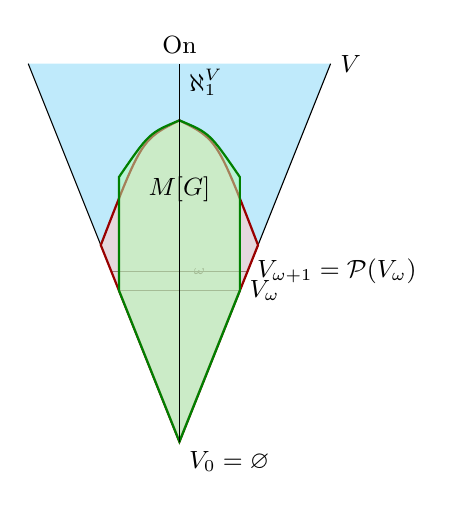
\begin{tikzpicture}[scale=0.16, every node/.style={font=\small}]
  \fill[cyan!25] (0,0) -- (12,30) -- (-12,30) -- cycle;
  \draw (12,30) -- (0,0) -- (-12,30);
  \node[right] at (12,30) {$V$};
  \node[below right] at (0,0) {$V_0 = \varnothing$};
  \draw (-4.8,12) -- (4.8,12) node[right] {$V_\omega$};
  \draw (-5.4,13.5) -- (5.4,13.5) node[right] {$V_{\omega+1} = \mathcal{P}(V_\omega)$};
  \node[right] at (0.3,13.5) {\tiny $\omega$};
  % red overhang: M[G] reaches wider than the ground model's cross-sections
  \fill[red!20, opacity=0.6] (0,0) -- (6.24,15.6) .. controls (3,24) .. (0,25.5)
      .. controls (-3,24) .. (-6.24,15.6) -- cycle;
  \draw[red!60!black, thick] (0,0) -- (6.24,15.6) .. controls (3,24) .. (0,25.5)
      .. controls (-3,24) .. (-6.24,15.6) -- cycle;
  % green M sitting inside
  \fill[green!30, opacity=0.5] (0,0) -- (4.8,12) -- (4.8,21)
      .. controls (2.4,24.5) .. (0,25.5) .. controls (-2.4,24.5) .. (-4.8,21) -- (-4.8,12) -- cycle;
  \draw[green!50!black, thick] (0,0) -- (4.8,12) -- (4.8,21)
      .. controls (2.4,24.5) .. (0,25.5) .. controls (-2.4,24.5) .. (-4.8,21) -- (-4.8,12) -- cycle;
  \node at (0,20) {$M[G]$};
  \draw (0,0) -- (0,30);
  \node[above] at (0,30) {$\mathrm{On}$};
  \node[right] at (0,28.5) {$\aleph_1^V$};
\end{tikzpicture}
\end{document}
